% 3D 艺术画的计算

\subsection{3D 艺术画}
(未完成, 用一张示意图说明如何用一张正常的图生成 3D 艺术画)
\begin{figure}[ht]
\centering
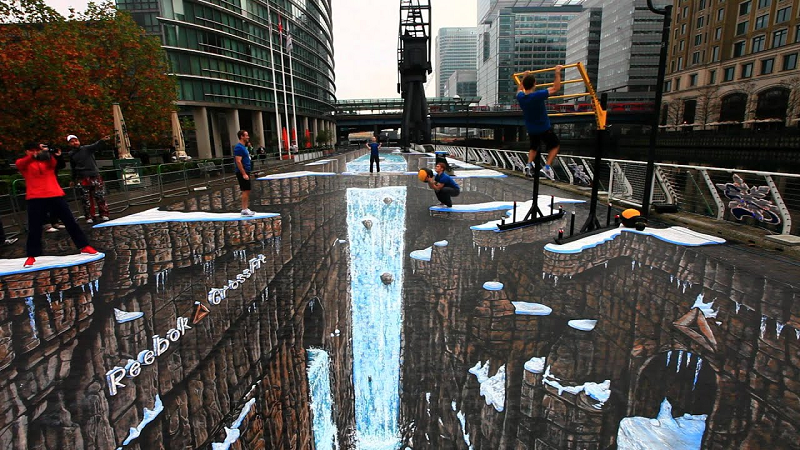
\includegraphics[width=10cm]{./figures/art3D_1.png}
\caption{2011 年最大的 3D 艺术画, 画于伦敦街头, 获吉尼斯纪录} \label{art3D_fig1}
\end{figure}

\begin{figure}[ht]
\centering
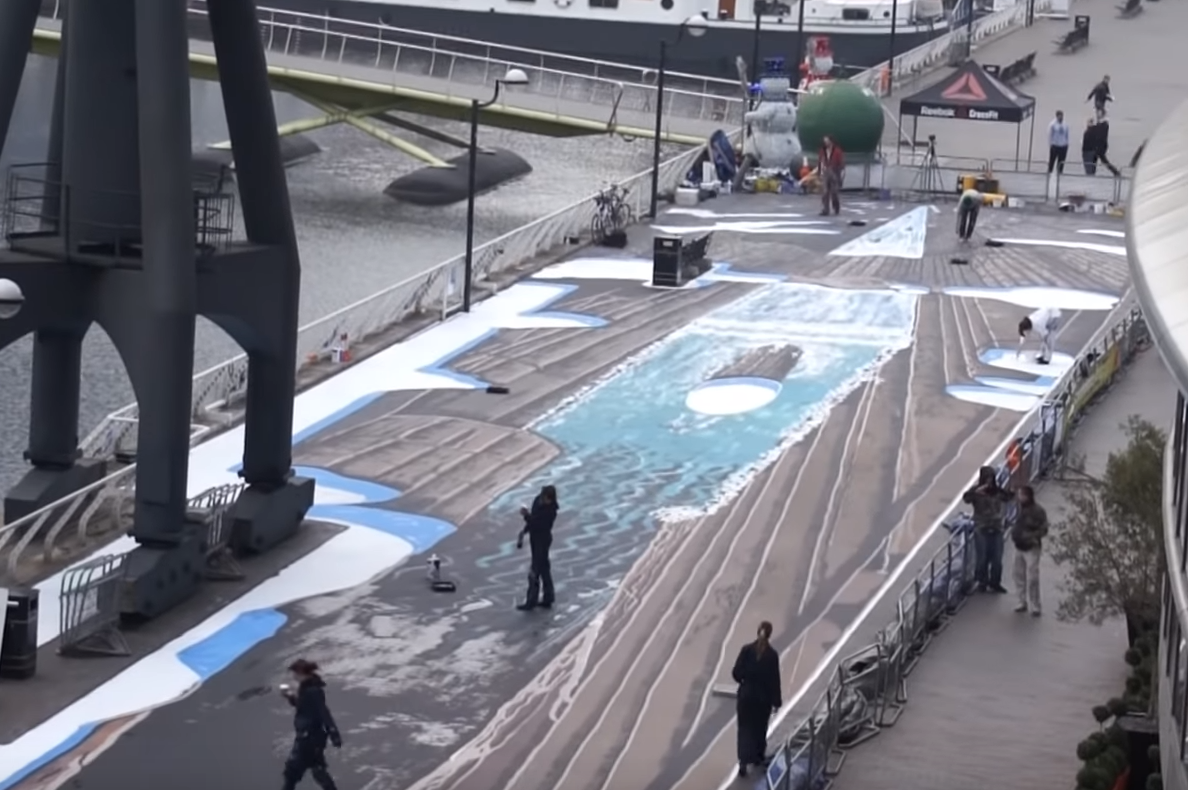
\includegraphics[width=10cm]{./figures/art3D_2.png}
\caption{从不同角度看 3D 艺术画(\autoref{art3D_fig1} 由该图中右上角相机拍摄)} \label{art3D_fig2}
\end{figure}


\subsection{计算}

\pentry{由图像坐标计算射线\upref{mn2lin}, 直线和平面的交点\upref{LPint}}

由预备知识中的两个词条, 若给出预期的效果图(即\autoref{art3D_fig1} 中的虚构部分), 世界坐标系中投影平面的位置, 以及相机模型的参数和位置, 就可以将效果图上的点一一对应到世界系的射线, 再对应到投影平面上.

我们不直接投影到世界系的 $xy$ 平面上, 是因为一些 3D 艺术画不仅使用地板, 也可能使用墙壁和天花板等多个平面.

(未完成: Matlab 代码)
